\newcommand\PD{\mathrm{PD}}
\renewcommand\FF{\mathcal{F}}

\begin{problem}[1]
  Using the algorithm described in class, compute the PD of the following simplexwise filtration:

  \begin{figure}[H]
    \centering

    \newcommand\defcoordinates{%
      \coordinate (a) at (0.1, 0.5);
      \coordinate (b) at (0.33, 0.8);
      \coordinate (c) at (0.66, 0.8);
      \coordinate (d) at (0.9, 0.5);
      \coordinate (e) at (0.5, 0.15);
    }

    \newcommand\plota{\filldraw[black] (a) circle (0.5pt) node[below] {$\scriptstyle a$};}
    \newcommand\plotb{\filldraw[black] (b) circle (0.5pt) node[above left] {$\scriptstyle b$};}
    \newcommand\plotc{\filldraw[black] (c) circle (0.5pt) node[above right] {$\scriptstyle c$};}
    \newcommand\plotd{\filldraw[black] (d) circle (0.5pt) node[below] {$\scriptstyle d$};}
    \newcommand\plote{\filldraw[black] (e) circle (0.5pt) node[below] {$\scriptstyle e$};}

    \newcommand\conab{\draw[black] (a) -- (b);}
    \newcommand\conbc{\draw[black] (b) -- (c);}
    \newcommand\concd{\draw[black] (c) -- (d);}
    \newcommand\conea{\draw[black] (e) -- (a);}
    \newcommand\coneb{\draw[black] (e) -- (b);}
    \newcommand\conec{\draw[black] (e) -- (c);}
    \newcommand\coned{\draw[black] (e) -- (d);}

    \newcommand\fillaeb{\fill[red, opacity=0.2] (a) -- (b) -- (e) -- cycle;}
    \newcommand\fillbec{\fill[red, opacity=0.2] (b) -- (e) -- (c) -- cycle;}
    \newcommand\fillced{\fill[red, opacity=0.2] (c) -- (e) -- (d) -- cycle;}

    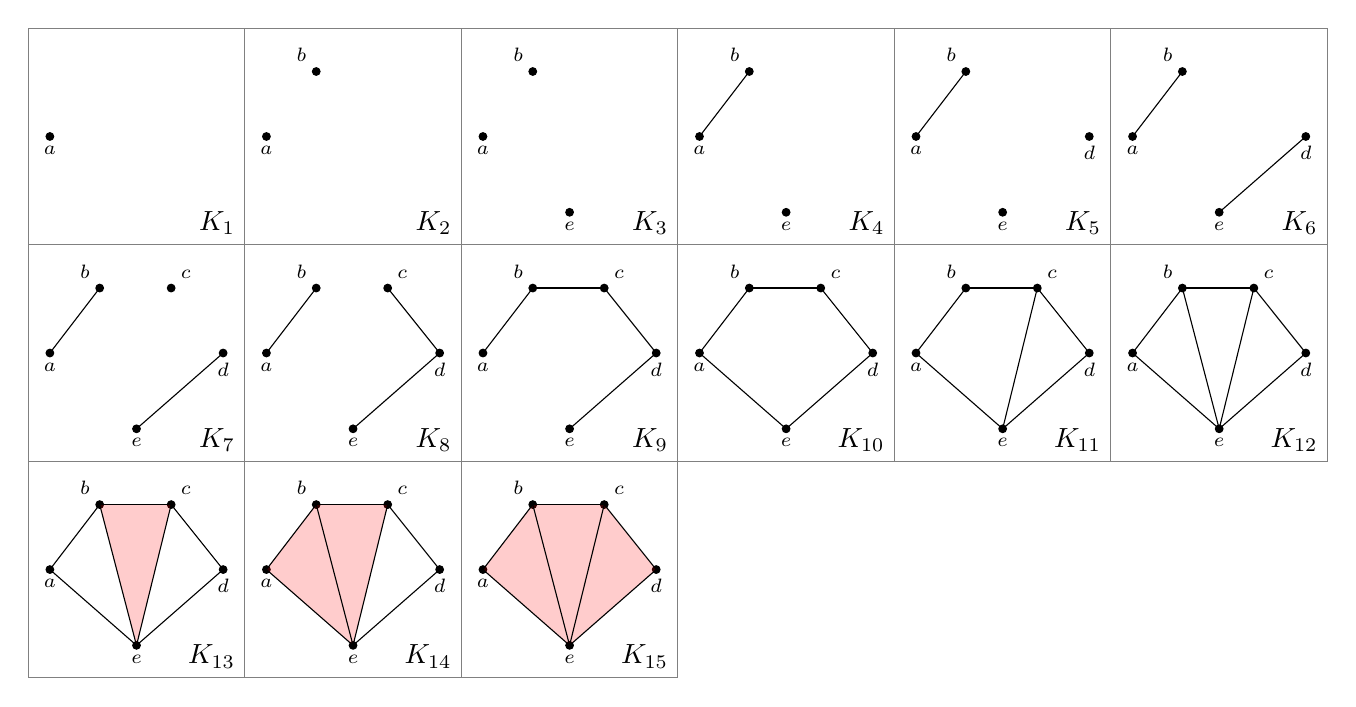
\begin{tikzpicture}
      % K1
      \begin{scope}[scale=2.75]
        \defcoordinates
        \draw[gray] (0,0) rectangle (1, 1);
        \node[anchor=south east] at (1, 0) {$K_1$};
        \plota
      \end{scope}

      % K2
      \begin{scope}[scale=2.75, shift={(1, 0)}]
        \defcoordinates
        \draw[gray] (0,0) rectangle (1, 1);
        \node[anchor=south east] at (1, 0) {$K_2$};
        \plota\plotb
      \end{scope}

      % K3
      \begin{scope}[scale=2.75, shift={(2, 0)}]
        \defcoordinates
        \draw[gray] (0,0) rectangle (1, 1);
        \node[anchor=south east] at (1, 0) {$K_3$};
        \plota\plotb\plote
      \end{scope}

      % K4
      \begin{scope}[scale=2.75, shift={(3, 0)}]
        \defcoordinates
        \draw[gray] (0,0) rectangle (1, 1);
        \node[anchor=south east] at (1, 0) {$K_4$};
        \plota\plotb\plote
        \conab
      \end{scope}

      % K5
      \begin{scope}[scale=2.75, shift={(4, 0)}]
        \defcoordinates
        \draw[gray] (0,0) rectangle (1, 1);
        \node[anchor=south east] at (1, 0) {$K_5$};
        \plota\plotb\plotd\plote
        \conab
      \end{scope}

      % K6
      \begin{scope}[scale=2.75, shift={(5, 0)}]
        \defcoordinates
        \draw[gray] (0,0) rectangle (1, 1);
        \node[anchor=south east] at (1, 0) {$K_6$};
        \plota\plotb\plotd\plote
        \conab\coned
      \end{scope}

      % K7
      \begin{scope}[scale=2.75, shift={(0, -1)}]
        \defcoordinates
        \draw[gray] (0,0) rectangle (1, 1);
        \node[anchor=south east] at (1, 0) {$K_7$};
        \plota\plotb\plotc\plotd\plote
        \conab\coned
      \end{scope}

      % K8
      \begin{scope}[scale=2.75, shift={(1, -1)}]
        \defcoordinates
        \draw[gray] (0,0) rectangle (1, 1);
        \node[anchor=south east] at (1, 0) {$K_8$};
        \plota\plotb\plotc\plotd\plote
        \conab\concd\coned
      \end{scope}

      % K9
      \begin{scope}[scale=2.75, shift={(2, -1)}]
        \defcoordinates
        \draw[gray] (0,0) rectangle (1, 1);
        \node[anchor=south east] at (1, 0) {$K_9$};
        \plota\plotb\plotc\plotd\plote
        \conab\conbc\concd\coned
      \end{scope}

      % K10
      \begin{scope}[scale=2.75, shift={(3, -1)}]
        \defcoordinates
        \draw[gray] (0,0) rectangle (1, 1);
        \node[anchor=south east] at (1, 0) {$K_{10}$};
        \plota\plotb\plotc\plotd\plote
        \conab\conbc\concd\conea\coned
      \end{scope}

      % K11
      \begin{scope}[scale=2.75, shift={(4, -1)}]
        \defcoordinates
        \draw[gray] (0,0) rectangle (1, 1);
        \node[anchor=south east] at (1, 0) {$K_{11}$};
        \plota\plotb\plotc\plotd\plote
        \conab\conbc\concd\conea\conec\coned
      \end{scope}

      % K12
      \begin{scope}[scale=2.75, shift={(5, -1)}]
        \defcoordinates
        \draw[gray] (0,0) rectangle (1, 1);
        \node[anchor=south east] at (1, 0) {$K_{12}$};
        \plota\plotb\plotc\plotd\plote
        \conab\conbc\concd\conea\coneb\conec\coned
      \end{scope}

      % K13
      \begin{scope}[scale=2.75, shift={(0, -2)}]
        \defcoordinates
        \draw[gray] (0,0) rectangle (1, 1);
        \node[anchor=south east] at (1, 0) {$K_{13}$};
        \plota\plotb\plotc\plotd\plote
        \fillbec
        \conab\conbc\concd\conea\coneb\conec\coned
      \end{scope}

      % K14
      \begin{scope}[scale=2.75, shift={(1, -2)}]
        \defcoordinates
        \draw[gray] (0,0) rectangle (1, 1);
        \node[anchor=south east] at (1, 0) {$K_{14}$};
        \plota\plotb\plotc\plotd\plote
        \fillaeb\fillbec
        \conab\conbc\concd\conea\coneb\conec\coned
      \end{scope}

      % K15
      \begin{scope}[scale=2.75, shift={(2, -2)}]
        \defcoordinates
        \draw[gray] (0,0) rectangle (1, 1);
        \node[anchor=south east] at (1, 0) {$K_{15}$};
        \plota\plotb\plotc\plotd\plote
        \fillaeb\fillbec\fillced
        \conab\conbc\concd\conea\coneb\conec\coned
      \end{scope}
    \end{tikzpicture}
  \end{figure}

  Specifically, provide intervals in the PD of each dimension and also for each finite interval (not ending with $+\infty$),  provide its representative (aka. its entry in the ``$\zeta$'' table as demonstrated in class). Notice that a representative (chain) should be denoted as a sum of $\sigma_i$'s as done in class, where $i$ is the index of the simplex added in the filtration. For example, the chain a $a + b$ should be denoted as $\sigma_1 + \sigma_2$ where $\sigma_1 = a$ and $\sigma_2 = b$.

  \textit{Remark:} There are several ways to quickly check whether your results make sense:
  \begin{enumerate}
    \item Each index should occur exactly once in an interval, either as the start or the end.

    \item The representative for an interval $[b, d)$ should be a cycle created in $K_b$ and becoming a boundary in $K_d$.
  \end{enumerate}
\end{problem}

\begin{solution}
  The PD is given by
  \begin{align*}
    \PD_0(\FF) &= \{(2, 4), (5, 6), (7, 8), (3, 9)\} \\
    \PD_1(\FF) &= \{(12, 13), (11, 14), (10, 15)\}
  .\end{align*}
  The $\zeta(i)$ table is given by
  \begin{equation*}
    \begin{tabular}[b]{c|l}
      i & $\zeta(i)$ \\
      \hline
      2 & $\sigma_1 + \sigma_2$ \\
      3 & $\sigma_2 + \sigma_3$ \\
      5 & $\sigma_3 + \sigma_5$ \\
      7 & $\sigma_5 + \sigma_7$ \\
      10 & $\sigma_6 + \sigma_8 + \sigma_{10}$ \\
      11 & $\sigma_4 + \sigma_9 + \sigma_{10} + \sigma_{11}$ \\
      12 & $\sigma_9 + \sigma_{11} + \sigma_{12}$ \\
    \end{tabular}\qedhere
  \end{equation*}
\end{solution}

\begin{problem}[2]
  Given a filtration $\FF$, its \textit{$p$-th Betti curve} $B_p : I \to \N$ is a map from the indices $I$ of the filtration $\FF$ to the natural numbers $\N$ such that $B_p(i)$ is the $p$-th Betti number of the complex $K_i$ in $\FF$. Compute the $0$th and $1$st  Betti curve for the filtration in Question 1. Specifically, fill out a table of the following form:

  \vspace{0.5em}

  \begin{tabular}{|c|c|c|c|c|}
    \hline
    Index & 1 & 2 & $\cdots$ & 15 \\
    \hline
    $B_0$ & & & & \\
    \hline
    $B_1$ & & & & \\
    \hline
  \end{tabular}

  \vspace{0.5em}

  \textit{Hint:} Recall that there is a way mentioned in class about reading off the Betti numbers for a complex in a filtration using the persistence diagram (barcode).
\end{problem}

\begin{solution}
  Graphing the Betti curves is a good way to visualize the Betti numbers. The $0$th Betti number counts the number of connected components, and the $1$st Betti number counts the number of holes in the complex. The Betti curves are shown below.
  \begin{figure}[H]
    \centering

    \begin{subfigure}[b]{\textwidth}
      \centering

      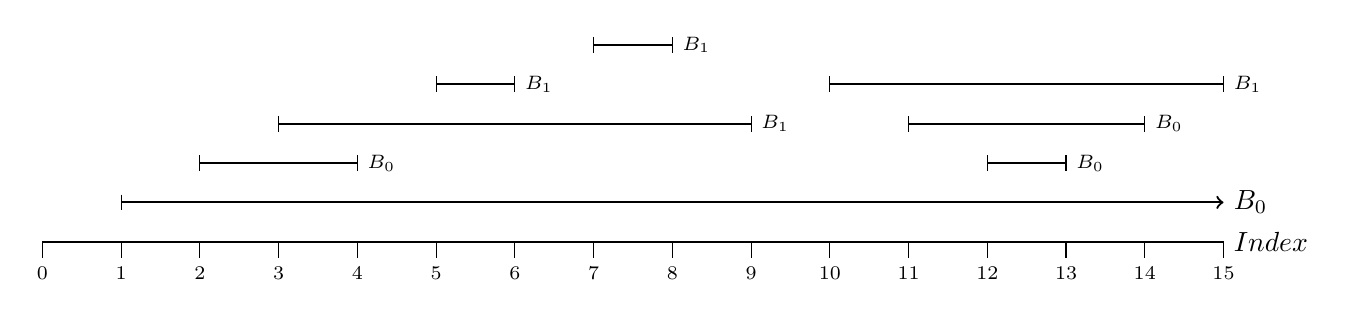
\begin{tikzpicture}
        % draw a line from 0 to 15 with ticks
        \draw[thick] (0, 0) -- (15, 0) node[right] {$\text{Index}$};
        \foreach \x in {0, 1, ..., 15} {
          \draw (\x, 0) -- (\x, -0.2) node[below] {$\scriptstyle \x$};
        }

        \draw[thick, ->] (1, 0.5) -- (15, 0.5) node[right] {$B_0$};
        \draw (1, 0.6) -- (1, 0.4);

        \draw[thick] (2, 1) -- (4, 1) node[right] {$\scriptstyle B_0$};
        \draw (2, 1.1) -- (2, 0.9);
        \draw (4, 1.1) -- (4, 0.9);

        \draw[thick] (12, 1) -- (13, 1) node[right] {$\scriptstyle B_0$};
        \draw (12, 1.1) -- (12, 0.9);
        \draw (13, 1.1) -- (13, 0.9);

        \draw[thick] (11, 1.5) -- (14, 1.5) node[right] {$\scriptstyle B_0$};
        \draw (11, 1.6) -- (11, 1.4);
        \draw (14, 1.6) -- (14, 1.4);

        \draw[thick] (3, 1.5) -- (9, 1.5) node[right] {$\scriptstyle B_1$};
        \draw (3, 1.6) -- (3, 1.4);
        \draw (9, 1.6) -- (9, 1.4);

        \draw[thick] (5, 2) -- (6, 2) node[right] {$\scriptstyle B_1$};
        \draw (5, 2.1) -- (5, 1.9);
        \draw (6, 2.1) -- (6, 1.9);

        \draw[thick] (10, 2) -- (15, 2) node[right] {$\scriptstyle B_1$};
        \draw (10, 2.1) -- (10, 1.9);
        \draw (15, 2.1) -- (15, 1.9);

        \draw[thick] (7, 2.5) -- (8, 2.5) node[right] {$\scriptstyle B_1$};
        \draw (7, 2.6) -- (7, 2.4);
        \draw (8, 2.6) -- (8, 2.4);
      \end{tikzpicture}
    \end{subfigure}

    \begin{subfigure}[b]{\textwidth}
    \end{subfigure}

    \begin{subfigure}[b]{\textwidth}
      \begin{equation*}
        \begin{tabular}[b]{|c|c|c|c|c|c|c|c|c|c|c|c|c|c|c|c|}
          \hline
          Index & 1 & 2 & 3 & 4 & 5 & 6 & 7 & 8 & 9 & 10 & 11 & 12 & 13 & 14 & 15 \\
          \hline
          $B_0$ & 1 & 2 & 3 & 2 & 3 & 2 & 3 & 2 & 1 & 1 & 1 & 1 & 1 & 1 & 1 \\
          \hline
          $B_1$ & 0 & 0 & 0 & 0 & 0 & 0 & 0 & 0 & 0 & 1 & 2 & 3 & 2 & 1 & 0 \\
          \hline
        \end{tabular}\qedhere
      \end{equation*}
    \end{subfigure}
  \end{figure}
\end{solution}

\begin{problem}[3]
  Consider the following non-simplex-wise filtration $\FF$ and its corresponding simplexwise filtration $\FF'$ where the dashed lines indicate equality of complexes:

  \begin{figure}[H]
    \centering
    \includegraphics[width=0.8\textwidth]{./image-files/homework-01/problem-03.png}
  \end{figure}

  Convert the following intervals in the PD of $\FF'$ to intervals in the PD of $\FF$ (if an interval does not have correspondence in $\FF$, just say ``none''):
  \begin{enumerate}
    \item $[2, 5)$

    \item $[7, 13)$

    \item $[2, 4)$
  \end{enumerate}
\end{problem}

\begin{solution}\leavevmode
  \begin{enumerate}
    \item From the diagram, we notice that $K_2' = K_1 \subset \FF$ and that $K_5'$ lies strictly before $K_4' = K_2 \subset \FF$. Therefore, the feature born at index $2$ in $\FF'$ is born in $K_1$ of $\FF$, and it dies before reaching $K_2$. Thus, the corresponding interval in $\FF$ is $[1, 2)$.

    \item We notice that $K_6' = K_3$ in $\FF$ and $K_7'$ immediately follows it, so $K_7'$ is contained within $K_3$. Also, we notice that $K_{13}' = K_6$ in $\FF$, so, its death occurs just before the inclusion into $K_6$. Therefore, the feature is born in $K_3$ and dies before entering $K_6$, giving the interval $[3, 6)$.

    \item Here, both $K_2'$ and $K_4'$ lie within $K_1$ of $\FF$. Since the entire birth-death interval lies strictly inside a single complex in $\FF$, this feature does not appear in the persistence diagram of $\FF$. Therefore, the corresponding interval in $\FF$ is ``none''.\qedhere
  \end{enumerate}
\end{solution}

\begin{problem}[4]
  Consider four points $a$, $b$, $c$, and $d$ with the following pair-wise distance:

  \vspace{0.5em}

  \begin{tabular}{|c|c|c|c|c|}
    \hline
    & $a$ & $b$ & $c$ & $d$ \\
    \hline
    $a$ & & 1.5 & 0.1 & 0.5 \\
    \hline
    $b$ & & & 1.0 & 0.3 \\
    \hline
    $c$ & & & & 0.9 \\
    \hline
    $d$ & & & & \\
    \hline
  \end{tabular}

  \vspace{0.5em}

  Construct the Vietoris-Rips filtration for the four points. You only need to list the different complexes in the filtration, by denoting each simplex as, say, $abcd$. (Recall that to build VR filtration, you only need to first figure out the order of the edges being introduced, and then you just take the clique complexes once you figure out the edges.)
\end{problem}

\begin{solution}
  The VR filtration is given by the following complexes:
  \begin{figure}[H]
    \centering

    \newcommand\defcoordinates{%
      \coordinate (a) at (0.25, 0.85);
      \coordinate (b) at (0.75, 0.3);
      \coordinate (c) at (0.25, 0.3);
      \coordinate (d) at (0.75, 0.85);
    }

    \newcommand\plota{\filldraw[black] (a) circle (0.5pt) node[above left] {$\scriptstyle a$};}
    \newcommand\plotb{\filldraw[black] (b) circle (0.5pt) node[below] {$\scriptstyle b$};}
    \newcommand\plotc{\filldraw[black] (c) circle (0.5pt) node[below] {$\scriptstyle c$};}
    \newcommand\plotd{\filldraw[black] (d) circle (0.5pt) node[above right] {$\scriptstyle d$};}

    \newcommand\conab{\draw[black] (a) -- (b);}
    \newcommand\conac{\draw[black] (a) -- (c);}
    \newcommand\conad{\draw[black] (a) -- (d);}
    \newcommand\conbc{\draw[black] (b) -- (c);}
    \newcommand\conbd{\draw[black] (b) -- (d);}
    \newcommand\concd{\draw[black] (c) -- (d);}

    \newcommand\fillcad{\fill[red, opacity=0.2] (c) -- (a) -- (d) -- cycle;}
    \newcommand\fillw{
      \fill[red, opacity=0.2] (c) -- (a) -- (b) -- cycle;
      \fill[red, opacity=0.2] (a) -- (b) -- (d) -- cycle;
    }

    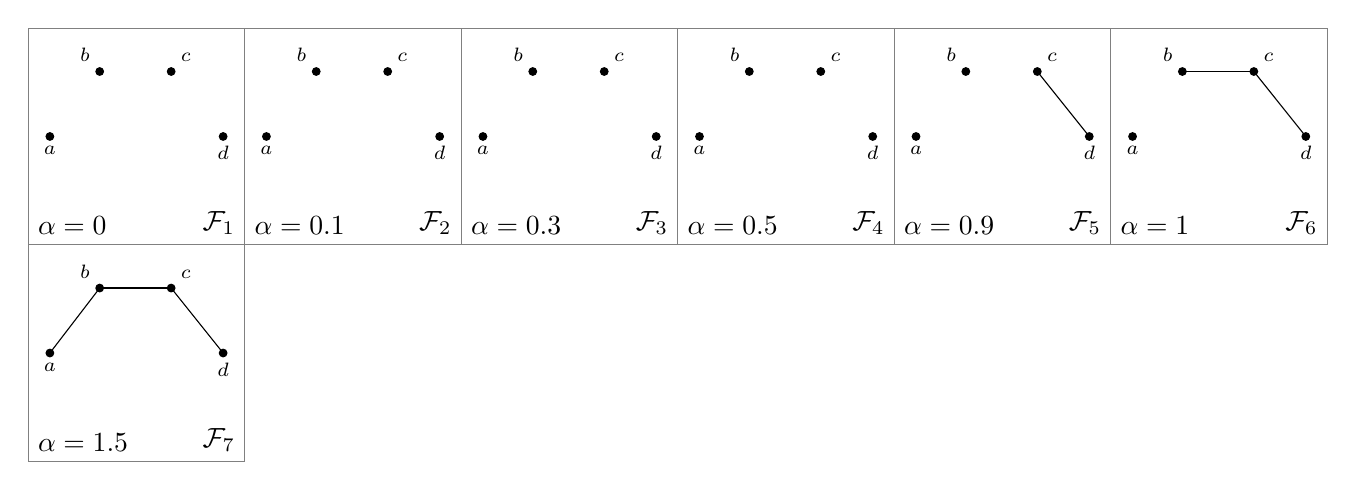
\begin{tikzpicture}
      % K1
      \begin{scope}[scale=2.75]
        \defcoordinates
        \draw[gray] (0,0) rectangle (1, 1);
        \node[anchor=south east] at (1, 0) {$\FF_1$};
        \node[anchor=south west] at (0, 0) {$\alpha = 0$};
        \plota\plotb\plotc\plotd
      \end{scope}

      % K2
      \begin{scope}[scale=2.75, shift={(1, 0)}]
        \defcoordinates
        \draw[gray] (0,0) rectangle (1, 1);
        \node[anchor=south east] at (1, 0) {$\FF_2$};
        \node[anchor=south west] at (0, 0) {$\alpha = 0.1$};
        \plota\plotb\plotc\plotd
        \conac
      \end{scope}

      % K3
      \begin{scope}[scale=2.75, shift={(2, 0)}]
        \defcoordinates
        \draw[gray] (0,0) rectangle (1, 1);
        \node[anchor=south east] at (1, 0) {$\FF_3$};
        \node[anchor=south west] at (0, 0) {$\alpha = 0.3$};
        \plota\plotb\plotc\plotd
        \conac\conbd
      \end{scope}

      % K4
      \begin{scope}[scale=2.75, shift={(3, 0)}]
        \defcoordinates
        \draw[gray] (0,0) rectangle (1, 1);
        \node[anchor=south east] at (1, 0) {$\FF_4$};
        \node[anchor=south west] at (0, 0) {$\alpha = 0.5$};
        \plota\plotb\plotc\plotd
        \conac\conbd\conad
      \end{scope}

      % K5
      \begin{scope}[scale=2.75, shift={(4, 0)}]
        \defcoordinates
        \draw[gray] (0,0) rectangle (1, 1);
        \node[anchor=south east] at (1, 0) {$\FF_5$};
        \node[anchor=south west] at (0, 0) {$\alpha = 0.9$};
        \plota\plotb\plotc\plotd
        \conac\conbd\conad\concd
        \fillcad
      \end{scope}

      % K6
      \begin{scope}[scale=2.75, shift={(5, 0)}]
        \defcoordinates
        \draw[gray] (0,0) rectangle (1, 1);
        \node[anchor=south east] at (1, 0) {$\FF_6$};
        \node[anchor=south west] at (0, 0) {$\alpha = 1$};
        \plota\plotb\plotc\plotd
        \conac\conbd\conad\concd\conbc
        \fillw
      \end{scope}

      % K7
      \begin{scope}[scale=2.75, shift={(0, -1)}]
        \defcoordinates
        \draw[gray] (0,0) rectangle (1, 1);
        \node[anchor=south east] at (1, 0) {$\FF_7$};
        \node[anchor=south west] at (0, 0) {$\alpha = 1.5$};
        \plota\plotb\plotc\plotd
        \conac\conbd\conad\concd\conbc\conab
        \fillw
      \end{scope}
    \end{tikzpicture}
  \end{figure}

  All the complexes from $\alpha = 0$ to $\alpha = 0.5$ are given by
  \begin{align*}
    \alpha = 0:& K_1 = \{a b, c, d\} \\
    \alpha = 0.1:& K_2 = \{a b, c, d, ac\} \\
    \alpha = 0.3:& K_3 = \{a b, c, d, ac, bd\} \\
    \alpha = 0.5:& K_4 = \{a b, c, d, ac, bd, ad\}
  .\end{align*}

  Then, at $\alpha = 0.9$, the triangle $acd$ is complete since we have the edges $ac$, $ad$, $cd$. Therefore,
  \[%
    K_5 = \{a b, c, d, ac, bd, ad, acd\}
  .\]%

  At $\alpha = 1$, the triangle $bcd$ is complete since we have the edges $bd$, $cd$, $bc$. Therefore,
  \[%
    K_6 = \{a b, c, d, ac, bd, ad, acd, bcd\}
  .\]%

  At $\alpha = 1.5$, the triangle $abd$ is complete since we have the edges $ab$, $ad$, $bd$. Also, another triangle is complete, $abc$, since we have the edges $ab$, $ac$, $bc$. Now the 3-simplex $abcd$ is present, since all 6 edges are in the complex. Therefore,
  \[%
    K_7 = \{a, b, c, d, ac, bd, ad, acd, bcd, abd, abc, abcd\}
  .\qedhere\]%
\end{solution}

\begin{problem}[5]
  \begin{figure}[H]
    \centering

    \begin{subfigure}[b]{0.45\textwidth}
      \centering

      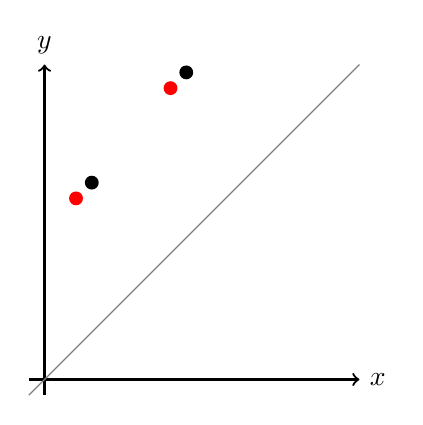
\begin{tikzpicture}
        \draw[thick, ->] (-0.2, 0) -- (4, 0) node[right] {$x$};
        \draw[thick, ->] (0, -0.2) -- (0, 4) node[above] {$y$};

        \draw[gray] (-0.2, -0.2) -- (4, 4);

        \begin{scope}[shift={(0, 1)}]
          \fill[red] (0.4, 1.3) circle (2.5pt);
          \fill[black] (0.6, 1.5) circle (2.5pt);

          \fill[red] (1.6, 2.7) circle (2.5pt);
          \fill[black] (1.8, 2.9) circle (2.5pt);
        \end{scope}
      \end{tikzpicture}
    \end{subfigure}
    \begin{subfigure}[b]{0.45\textwidth}
      \centering

      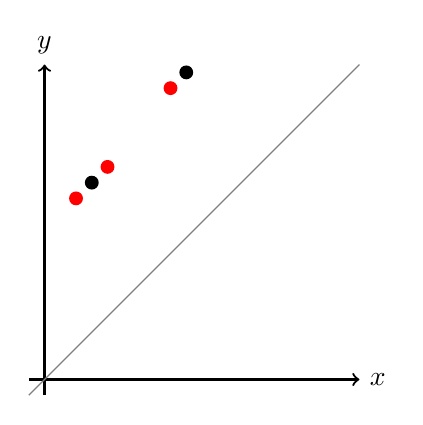
\begin{tikzpicture}
        \draw[thick, ->] (-0.2, 0) -- (4, 0) node[right] {$x$};
        \draw[thick, ->] (0, -0.2) -- (0, 4) node[above] {$y$};

        \draw[gray] (-0.2, -0.2) -- (4, 4);

        \begin{scope}[shift={(0, 1)}]
          \fill[red] (0.4, 1.3) circle (2.5pt);
          \fill[black] (0.6, 1.5) circle (2.5pt);
          \fill[red] (0.8, 1.7) circle (2.5pt);

          \fill[red] (1.6, 2.7) circle (2.5pt);
          \fill[black] (1.8, 2.9) circle (2.5pt);
        \end{scope}
      \end{tikzpicture}
    \end{subfigure}
  \end{figure}

  Consider the two PDs on the left $\R^2$ plane where one PD contains red points and another PD contains black points. Assume the following:
  \begin{enumerate}
    \item Each red or black point (interval) has the same length (aka. $d - b$) of 1.0.

    \item The first red point and the first black point are 0.2 distance away, and the second red point and the second black point are 0.2 distance away.

    \item The first black point and the second red points are 1.5 distance away.
  \end{enumerate}

  We then have that, the two PDs (on the left $\R^2$ plane) have a bottleneck distance of 0.2, with the two closest pairs of red and black points perfectly matched.

  Now, add another red point whose length is also 1.0 and whose distance to the first black point is 0.2, as indicated in right figure. What is the bottleneck distance of the two PDs in this case? You should also provide brief justifications for your answer.
\end{problem}

\begin{solution}
  In the original persistence diagrams (PDs), each red point can be perfectly matched to a black point with distance 0.2, and the bottleneck distance is 0.2. After adding a third red point in the right figure, there are now three red points and only two black points. Since the bottleneck distance involves computing a matching between the points in the two PDs (allowing unmatched points to be matched to the diagonal), we now must match one red point to the diagonal because there are more red points than black ones.

  There are two possible matchings. The two black points are still matched to the two closest red points at distance 0.2 or the extra red point must be matched to the diagonal. Its birth-death pair has length 1.0. In bottleneck distance, we take the maximum over the distances in the optimal matching. In this case, the distances are $\{0.2, 0.2, 1\}$. Thus, the bottleneck distance is the maximum of these, which is 1.

  Since we are allowed to match extra points to the diagonal, and this red point is unmatched (there are not enough black points), its best possible match is to the diagonal, which incurs a cost of 1. The optimal matching minimizes the maximum of the matching distances, so the bottleneck distance increases from 0.2 to 1.
\end{solution}
